\section{设计思路}

\subsection{DeepFM}

本算法主要基于Guo等人的DeepFM模型\cite{guoDeepFMFactorizationMachineBased2017}进行改进。
自DeepFM模型提出以来,
迅速在推荐系统领域成为最受欢迎的算法之一,
其主要基于Google的Wide \& Deep模型,
将Wide部分使用FM进行特征提取,
获得了不错的性能同时也有较高的准确率。
其算法的主要结构如\cref{fig:deepfm}所示。

\begin{figure}[!htbp]
	\centering
	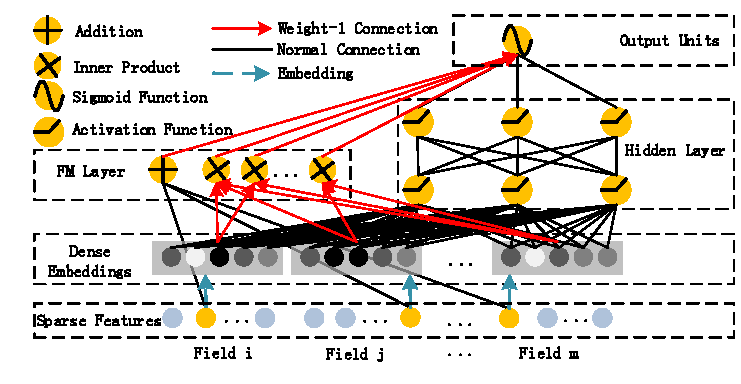
\includegraphics[width=.9\textwidth]{images/architecture-deepfm.pdf}
	\caption{DeepFM}\label{fig:deepfm}
\end{figure}

其主要用于对离散型变量进行训练。
将OneHot编码使用嵌入层嵌入后分别用FM和DNN进行训练,
最终FM和DNN的结果相加后输出。

但是在游戏推荐领域,
往往有非常多的标签数据、
连续型数据例如游玩时间等。
如果使用DeepFM模型,
往往会造成模型过于庞大的问题,
对于大量用户产生的数据,
往往会由于模型复杂度提升而耗费大量的计算资源,
对于对服务器有一定要求的游戏领域往往需要
额外的大量计算资源进行模型的训练。
上述问题均是DeepFM所无法解决的,
因此需要一种新的算法来进行优化,
以尽可能减少计算资源。

